\documentclass[../document.tex]{subfiles}
\begin{document}
\subsection{Robustness}
To test is robustness we will create custom patches with different features, walls/bumps/ramps, and test the model prediction against the real robot advancement obtained from the simulator. We always used a \emph{threhold} of $20$cm and a time window of two seconds. 
\subsubsection{Wall in front of Krock}
The easiest test we can perform is to place a wall in front of \emph{Krock}. If we place the wall at a different distance from the Krock's head we should reach a point where moving the wall towards the end of the patch, the model should predict traversable even if the wall itself is tall. Why? Because the robot will be able to traverse more than the threshold before being stopped by the wall.

We create fifty-five different patches by first placing the wall exactly in front of the robot and then move it $1$cm at the time towards the end. It follows some of the input patches ordered by distance from the robot.
\begin{figure}[H]
    \centering
    \begin{subfigure}[b]{0.160\textwidth}
    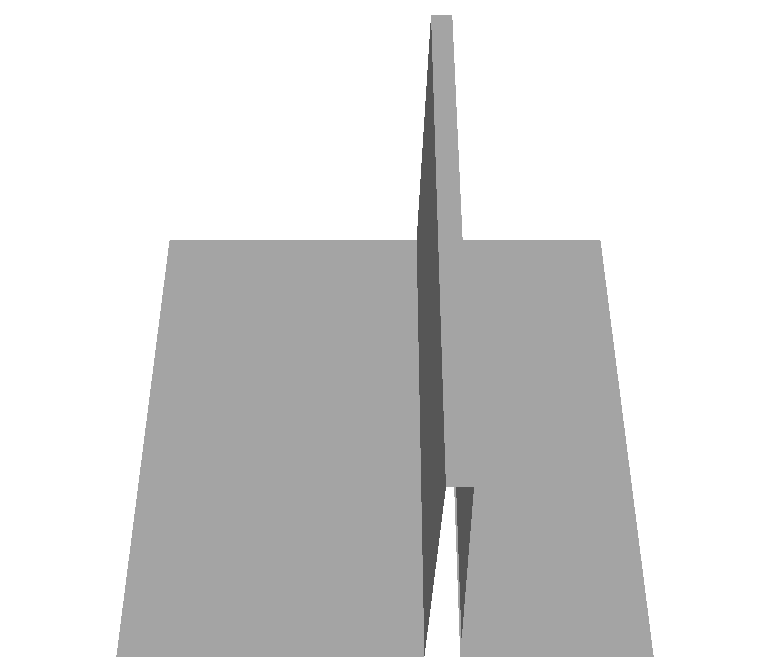
\includegraphics[width=\linewidth]{../img/5/custom_patches/walls_front/all/55-3d.png}
    \end{subfigure}
    \begin{subfigure}[b]{0.160\textwidth}
    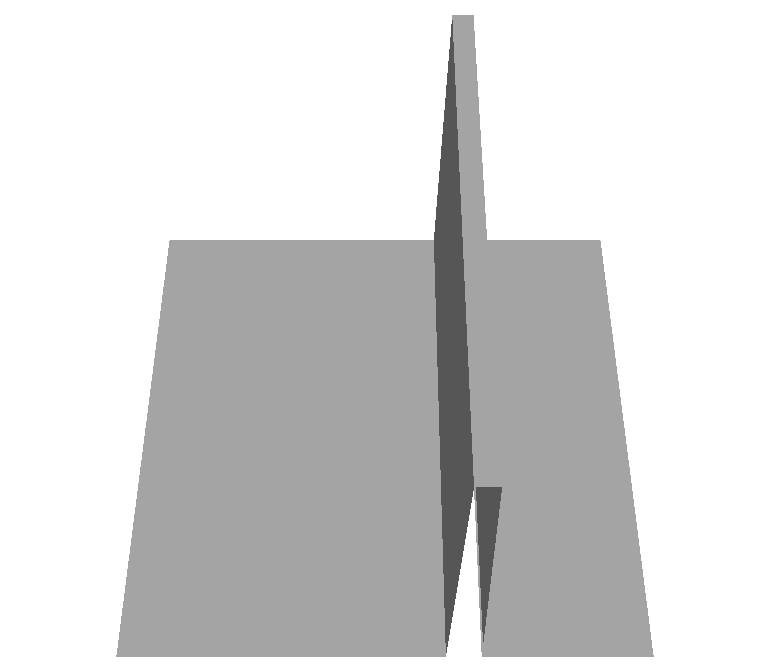
\includegraphics[width=\linewidth]{../img/5/custom_patches/walls_front/all/50-3d.png}
    \end{subfigure}
    \begin{subfigure}[b]{0.160\textwidth}
    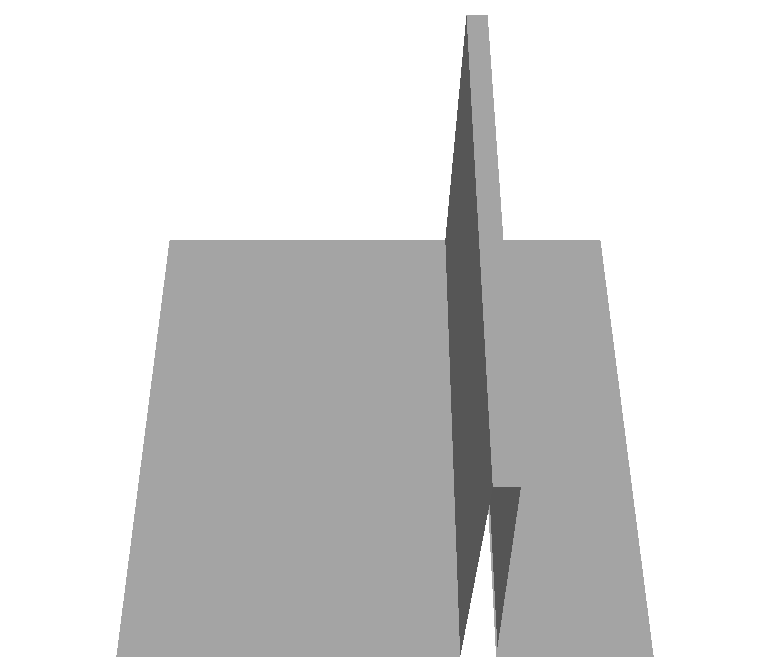
\includegraphics[width=\linewidth]{../img/5/custom_patches/walls_front/all/45-3d.png}
    \end{subfigure}
    \begin{subfigure}[b]{0.160\textwidth}
    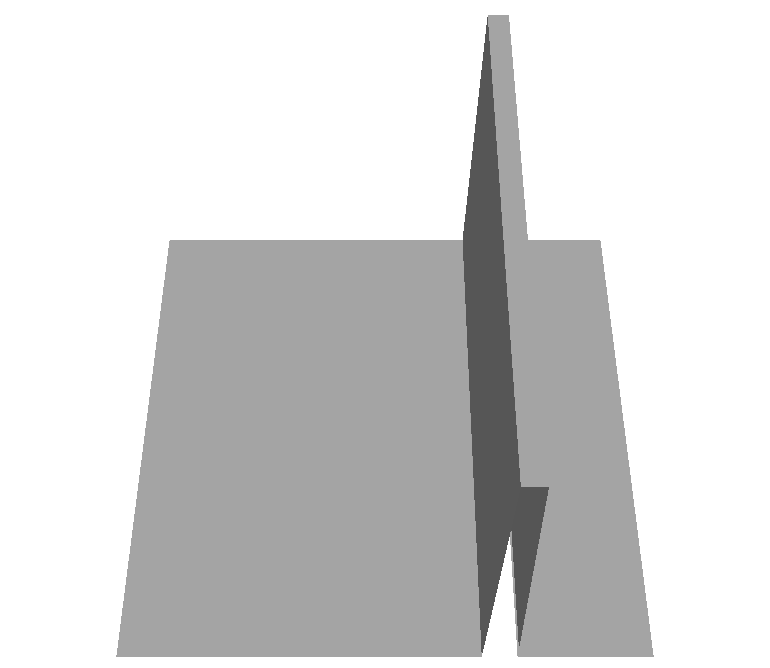
\includegraphics[width=\linewidth]{../img/5/custom_patches/walls_front/all/40-3d.png}
    \end{subfigure}
    \begin{subfigure}[b]{0.160\textwidth}
    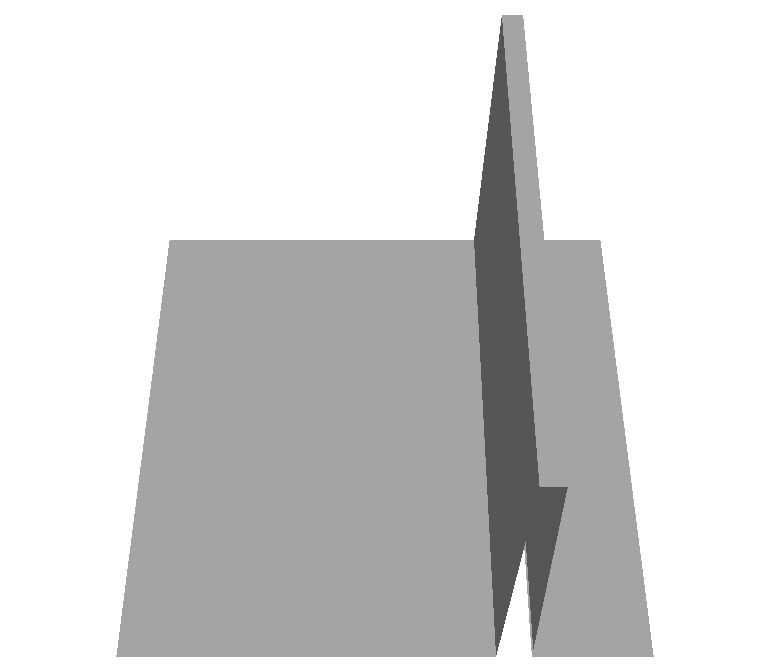
\includegraphics[width=\linewidth]{../img/5/custom_patches/walls_front/all/35-3d.png}
    \end{subfigure}
    \begin{subfigure}[b]{0.160\textwidth}
    \includegraphics[width=\linewidth]{../img/5/custom_patches/walls_front/all/30-3d.png}
    \end{subfigure}
    \begin{subfigure}[b]{0.160\textwidth}
    \includegraphics[width=\linewidth]{../img/5/custom_patches/walls_front/all/25-3d.png}
    \end{subfigure}
    \begin{subfigure}[b]{0.160\textwidth}
    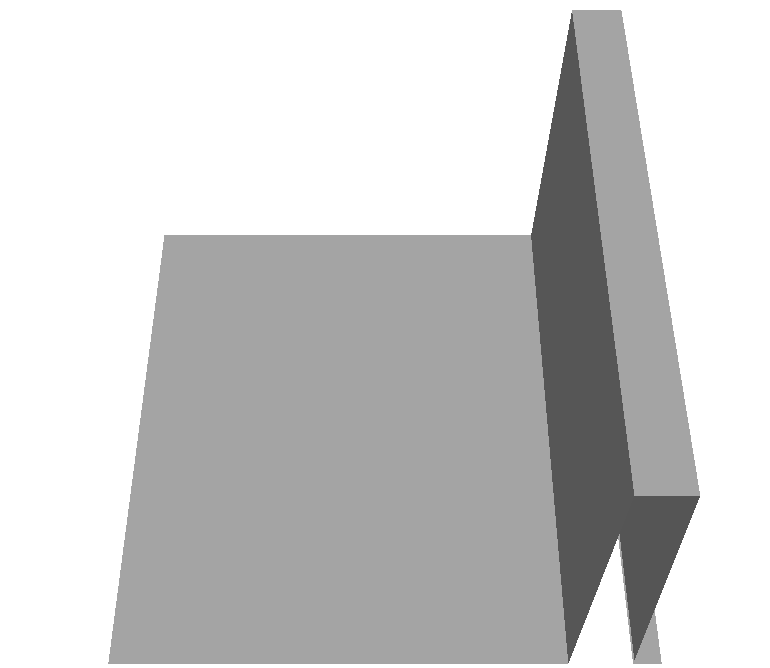
\includegraphics[width=\linewidth]{../img/5/custom_patches/walls_front/all/20-3d.png}
    \end{subfigure}
    \begin{subfigure}[b]{0.160\textwidth}
    \includegraphics[width=\linewidth]{../img/5/custom_patches/walls_front/all/15-3d.png}
    \end{subfigure}
    \begin{subfigure}[b]{0.160\textwidth}
    \includegraphics[width=\linewidth]{../img/5/custom_patches/walls_front/all/05-3d.png}
    \end{subfigure}
    \caption{Tested patches with $1$m wall at increasing distance from Krock.}
    \end{figure}

Given those inputs to the model, we get the following predictions

\begin{table}[H]
    \centering
    \begin{tabular}{l|cc}
        Distance(cm) & Prediction \\ 
        \hline
        0 - 19  & Not traversable \\ 
        19 - end & Traversable \\ 
        \hline
    \end{tabular}
    \caption{Model prediction from the wall patches}
\end{table}
To be sure the results are correct, we run the last not traversable patch and the first traversable
on the simulator to get real advancement. In the simulator, Krock advances $19.9$cm on the not traversable patch $(a)$ where the wall is at a distance of $19.6$cm from the head. While, on the first traversable where the wall is at a distance of $20.5$cm, the robot was able to travel for $22.4$. This shows that the model was able to correctly understand that the distance from the obstacle is more relevant than its height.
\begin{figure}[H]
    \centering
    \begin{subfigure}[b]{0.33\textwidth}
        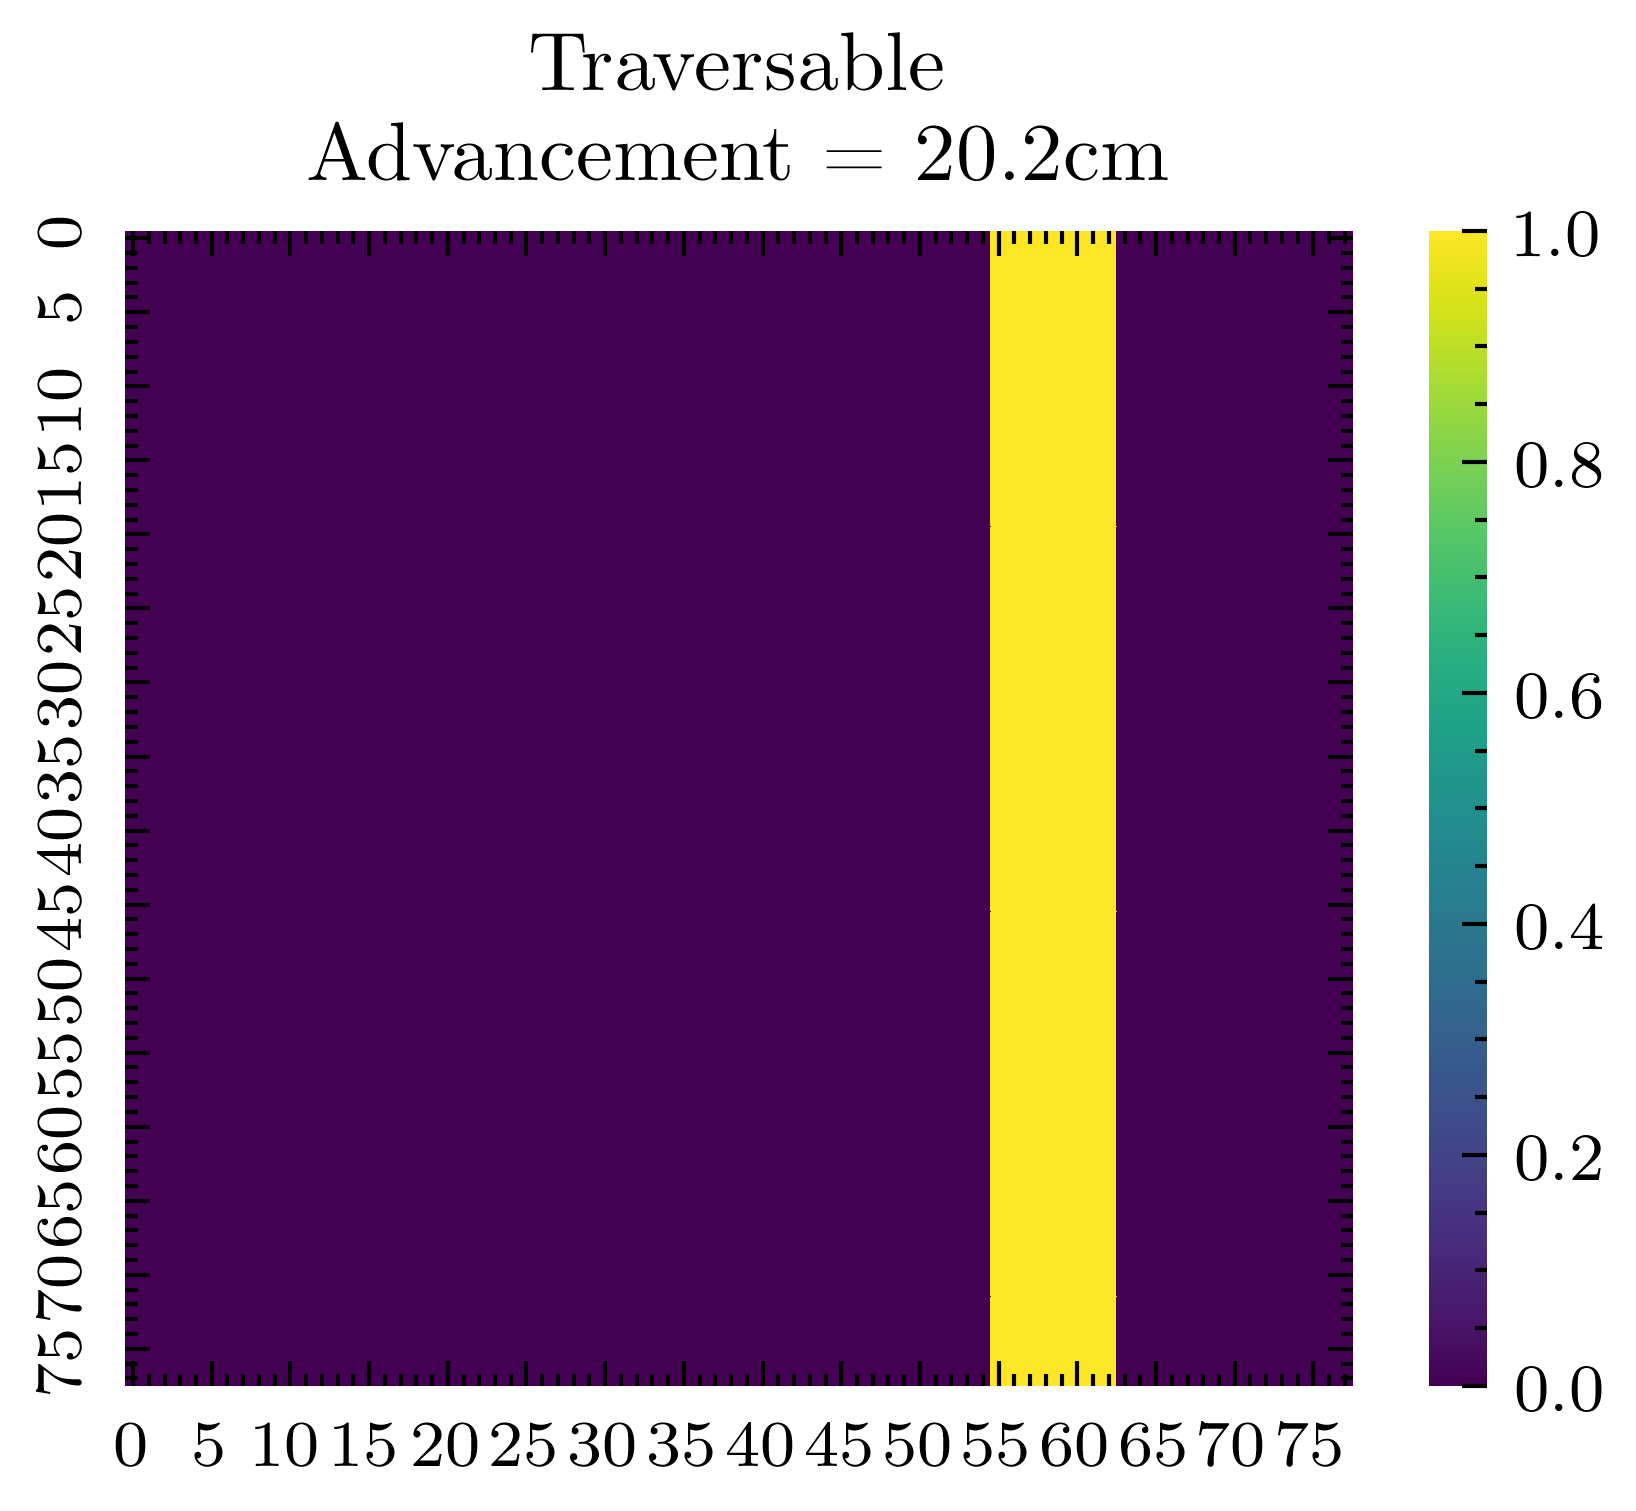
\includegraphics[width=\linewidth]{../img/5/custom_patches/walls_front/1-2d.png}
        \end{subfigure}   
    \begin{subfigure}[b]{0.33\textwidth}
        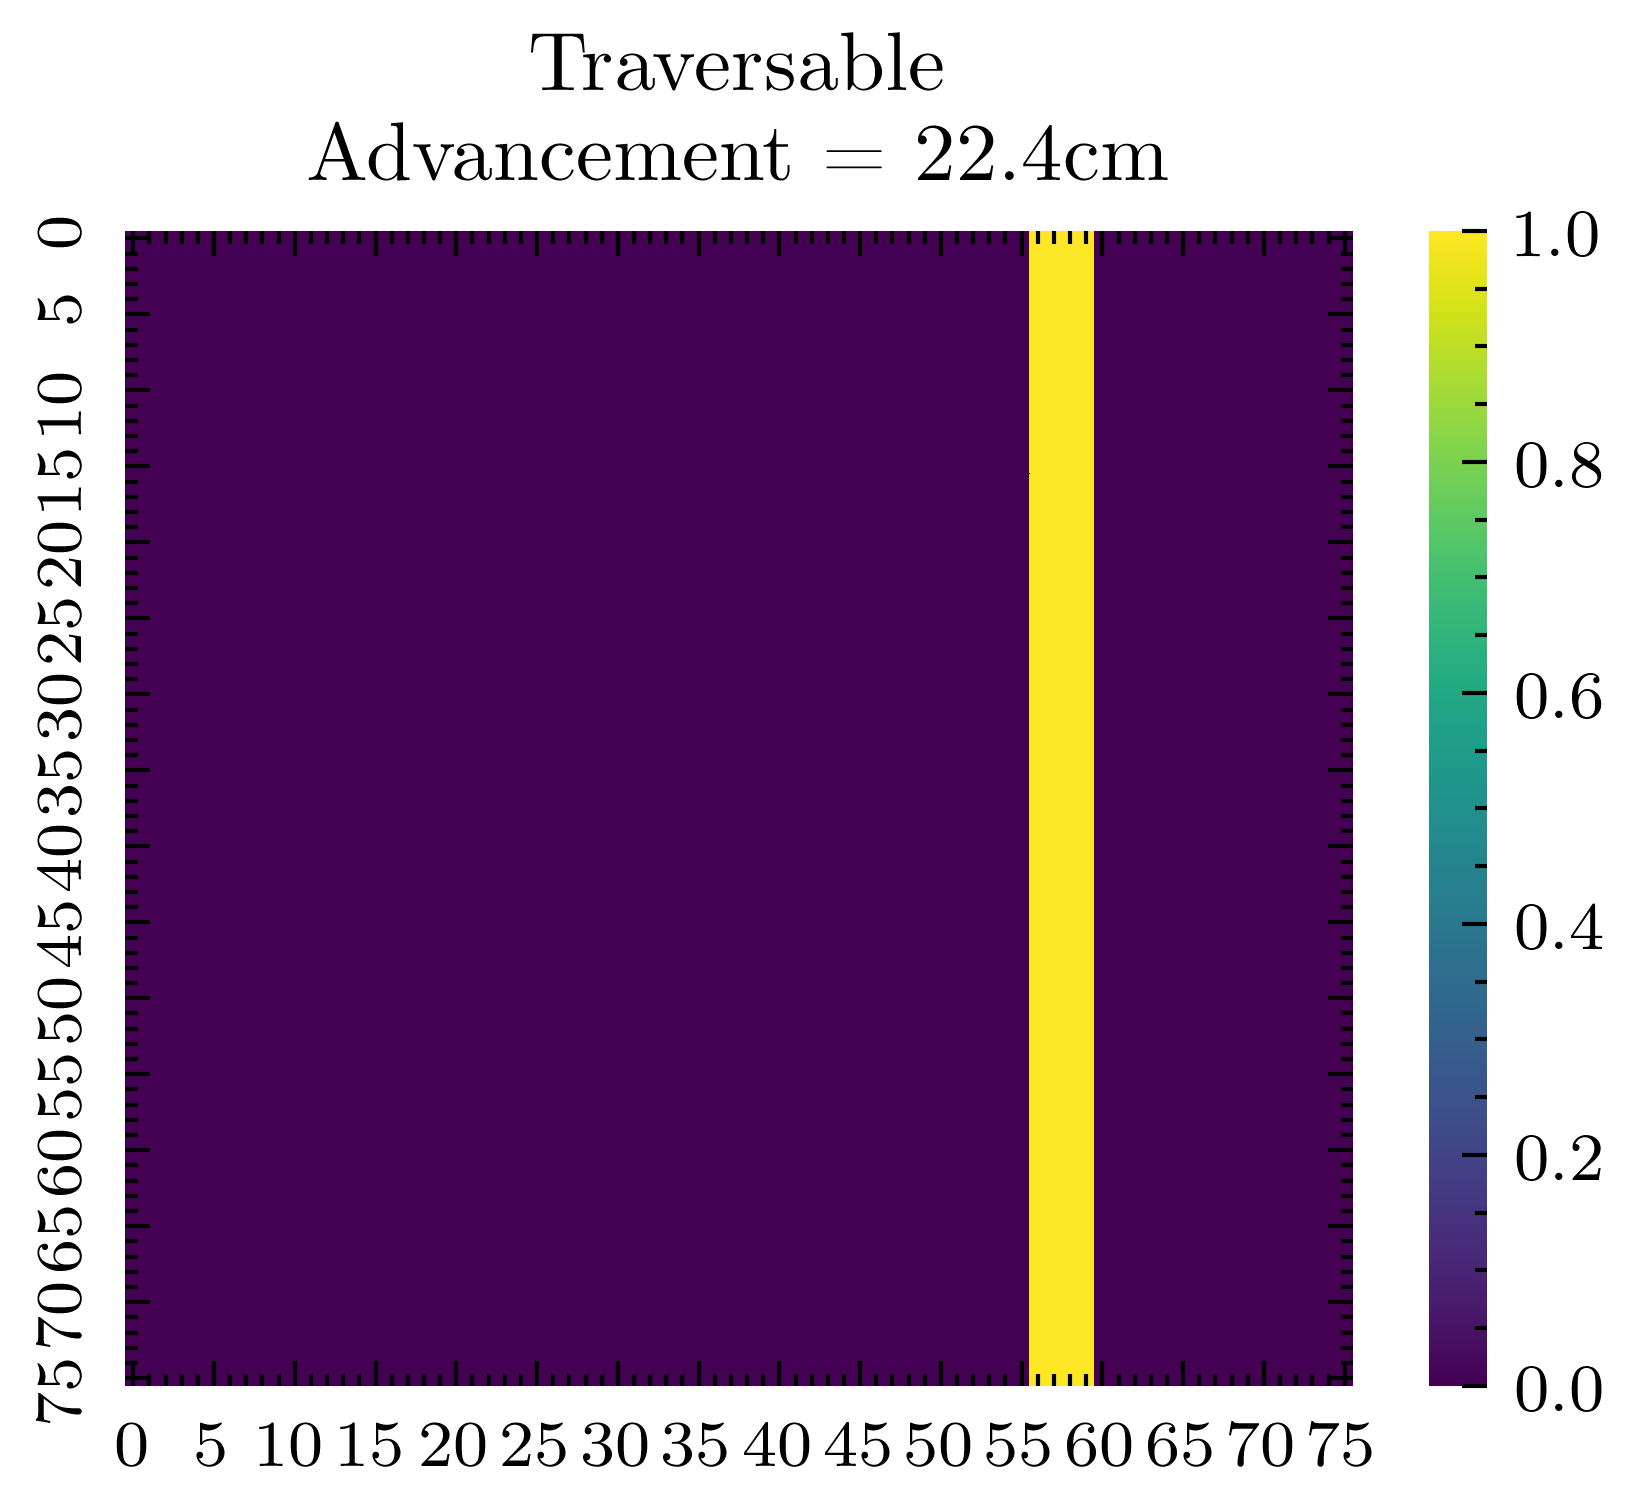
\includegraphics[width=\linewidth]{../img/5/custom_patches/walls_front/2-2d.png}
    \end{subfigure}   \\
    \begin{subfigure}[b]{0.33\textwidth}
        
\includegraphics[width=\linewidth]{../img/5/custom_patches/walls_front/1-3d.png}
        \caption{Distance  $19.6$cm}
    \end{subfigure}   
    \begin{subfigure}[b]{0.33\textwidth}
        
\includegraphics[width=\linewidth]{../img/5/custom_patches/walls_front/1-3d.png}
        \caption{Distance $20.5$cm}
    \end{subfigure}   
\end{figure}
Due to the patch resolution and some luck, the robot may advance more than the distance between its head and the wall. 

Furthermore, we can increase the wall size of the first traversable patch, $(b)$, to $10$ and to $100$m to stress even more the ability of the network to look at the distance and not at the height.

\begin{figure}[H]
    \centering
    \begin{subfigure}[b]{0.33\textwidth}
        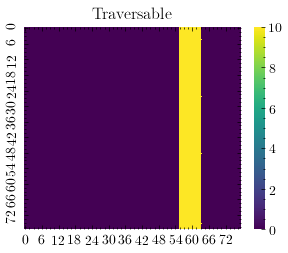
\includegraphics[width=\linewidth]{../img/5/custom_patches/walls_front/big-1-2d.png}
    \caption{height $=10$m}
    \end{subfigure}   
    \begin{subfigure}[b]{0.33\textwidth}
        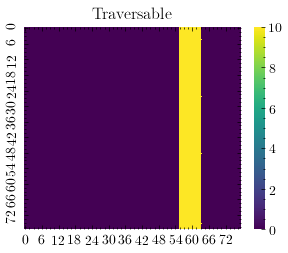
\includegraphics[width=\linewidth]{../img/5/custom_patches/walls_front/big-1-2d.png}
        \caption{height $=100$m}
    \end{subfigure}   
\caption{Traversable patches with a very tall wall.}    
\end{figure}
Correctly, the model classifies the patches as traversable and was not confused by the enourmous height of the wall.

\subsubsection{Increasing height walls}
We will test our model's robustness by placing different wall ahead of increasing heights ahead to check whether the prediction matches the output from the simulator. We run forty patches in the simulator from a wall'height of $1$cm to $20$cm. Krock's height from the ground is $4$cm. The following figure shows some of the inputs.

\begin{figure}[H]
    \centering
    \begin{subfigure}[b]{0.160\textwidth}
    \includegraphics[width=\linewidth]{/home/francesco/Documents/Master-Thesis/papers/Thesis/img/5/custom_patches/walls_increasing/all/00-3d.png}
    \end{subfigure}
    \begin{subfigure}[b]{0.160\textwidth}
    \includegraphics[width=\linewidth]{/home/francesco/Documents/Master-Thesis/papers/Thesis/img/5/custom_patches/walls_increasing/all/05-3d.png}
    \end{subfigure}
    \begin{subfigure}[b]{0.160\textwidth}
    \includegraphics[width=\linewidth]{/home/francesco/Documents/Master-Thesis/papers/Thesis/img/5/custom_patches/walls_increasing/all/10-3d.png}
    \end{subfigure}
    \begin{subfigure}[b]{0.160\textwidth}
    \includegraphics[width=\linewidth]{/home/francesco/Documents/Master-Thesis/papers/Thesis/img/5/custom_patches/walls_increasing/all/15-3d.png}
    \end{subfigure}
    \begin{subfigure}[b]{0.160\textwidth}
    \includegraphics[width=\linewidth]{/home/francesco/Documents/Master-Thesis/papers/Thesis/img/5/custom_patches/walls_increasing/all/20-3d.png}
    \end{subfigure}
    \begin{subfigure}[b]{0.160\textwidth}
    \includegraphics[width=\linewidth]{/home/francesco/Documents/Master-Thesis/papers/Thesis/img/5/custom_patches/walls_increasing/all/25-3d.png}
    \end{subfigure}
    \begin{subfigure}[b]{0.160\textwidth}
    \includegraphics[width=\linewidth]{/home/francesco/Documents/Master-Thesis/papers/Thesis/img/5/custom_patches/walls_increasing/all/30-3d.png}
    \end{subfigure}
    \begin{subfigure}[b]{0.160\textwidth}
    \includegraphics[width=\linewidth]{/home/francesco/Documents/Master-Thesis/papers/Thesis/img/5/custom_patches/walls_increasing/all/35-3d.png}
    \end{subfigure}
    \caption{Tested patches with a wall at increasing height ahead Krock.}
    \end{figure}
The models predicts that the walls under $10$cm are traversable.
\begin{table}[H]
    \centering
    \begin{tabular}{l|cc}
        Height(cm) & Prediction \\ 
        \hline
        0 - 10  & Traversable \\ 
        10 - end & Not Traversable \\ 
        \hline
    \end{tabular}
    \caption{Model prediction from the wall patches}
\end{table}
We can compare the model's prediction with the advancement computed in the simulator using the same approach from the last section. The following figure shows the results from the last traversable patch and the first non traversable.

\begin{figure}[H]
    \centering
    \begin{subfigure}[b]{0.33\textwidth}
        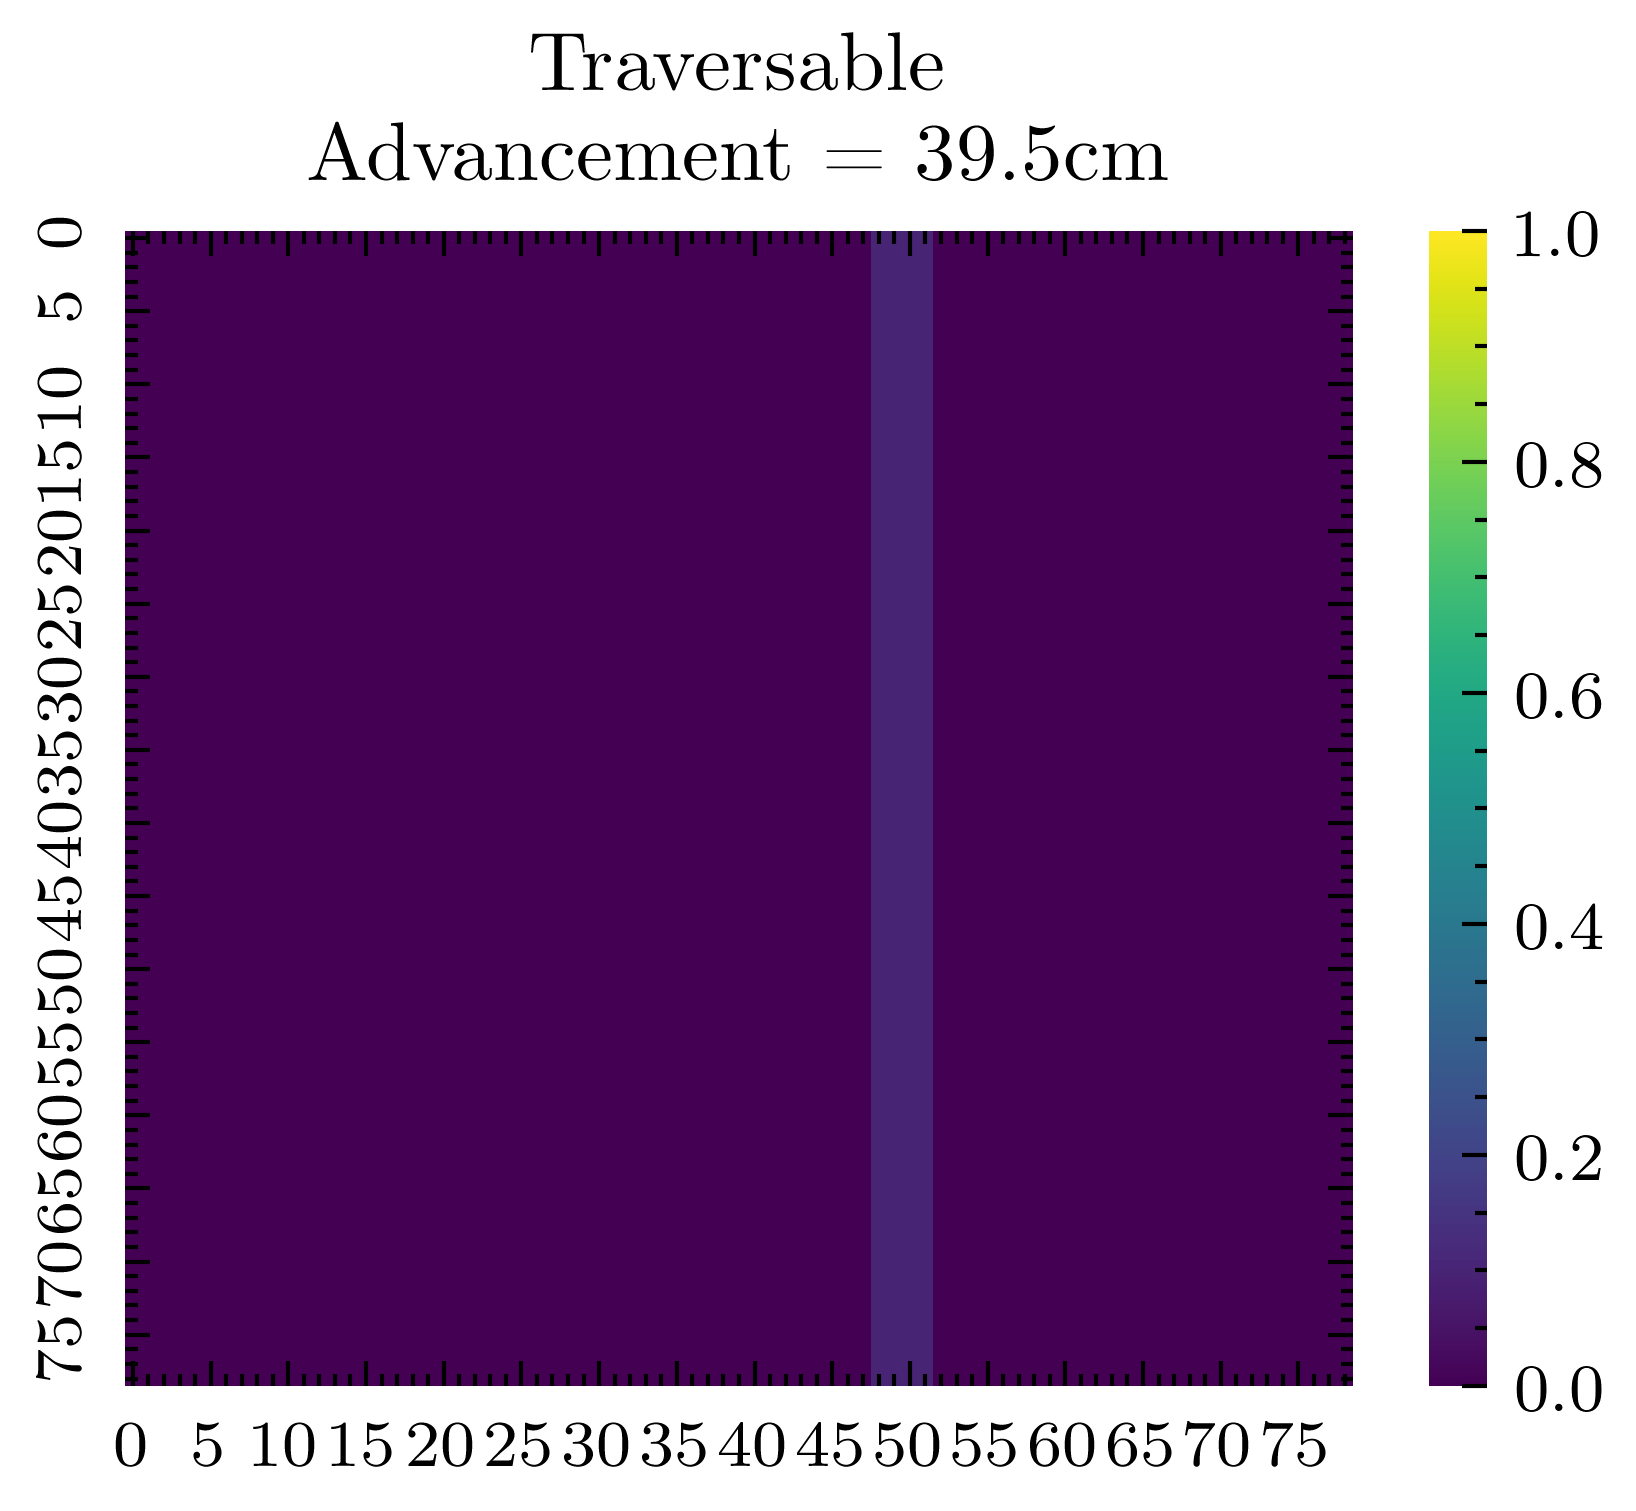
\includegraphics[width=\linewidth]{../img/5/custom_patches/walls_increasing/wall-height-1-2d.png}
    \end{subfigure}   
    \begin{subfigure}[b]{0.33\textwidth}
        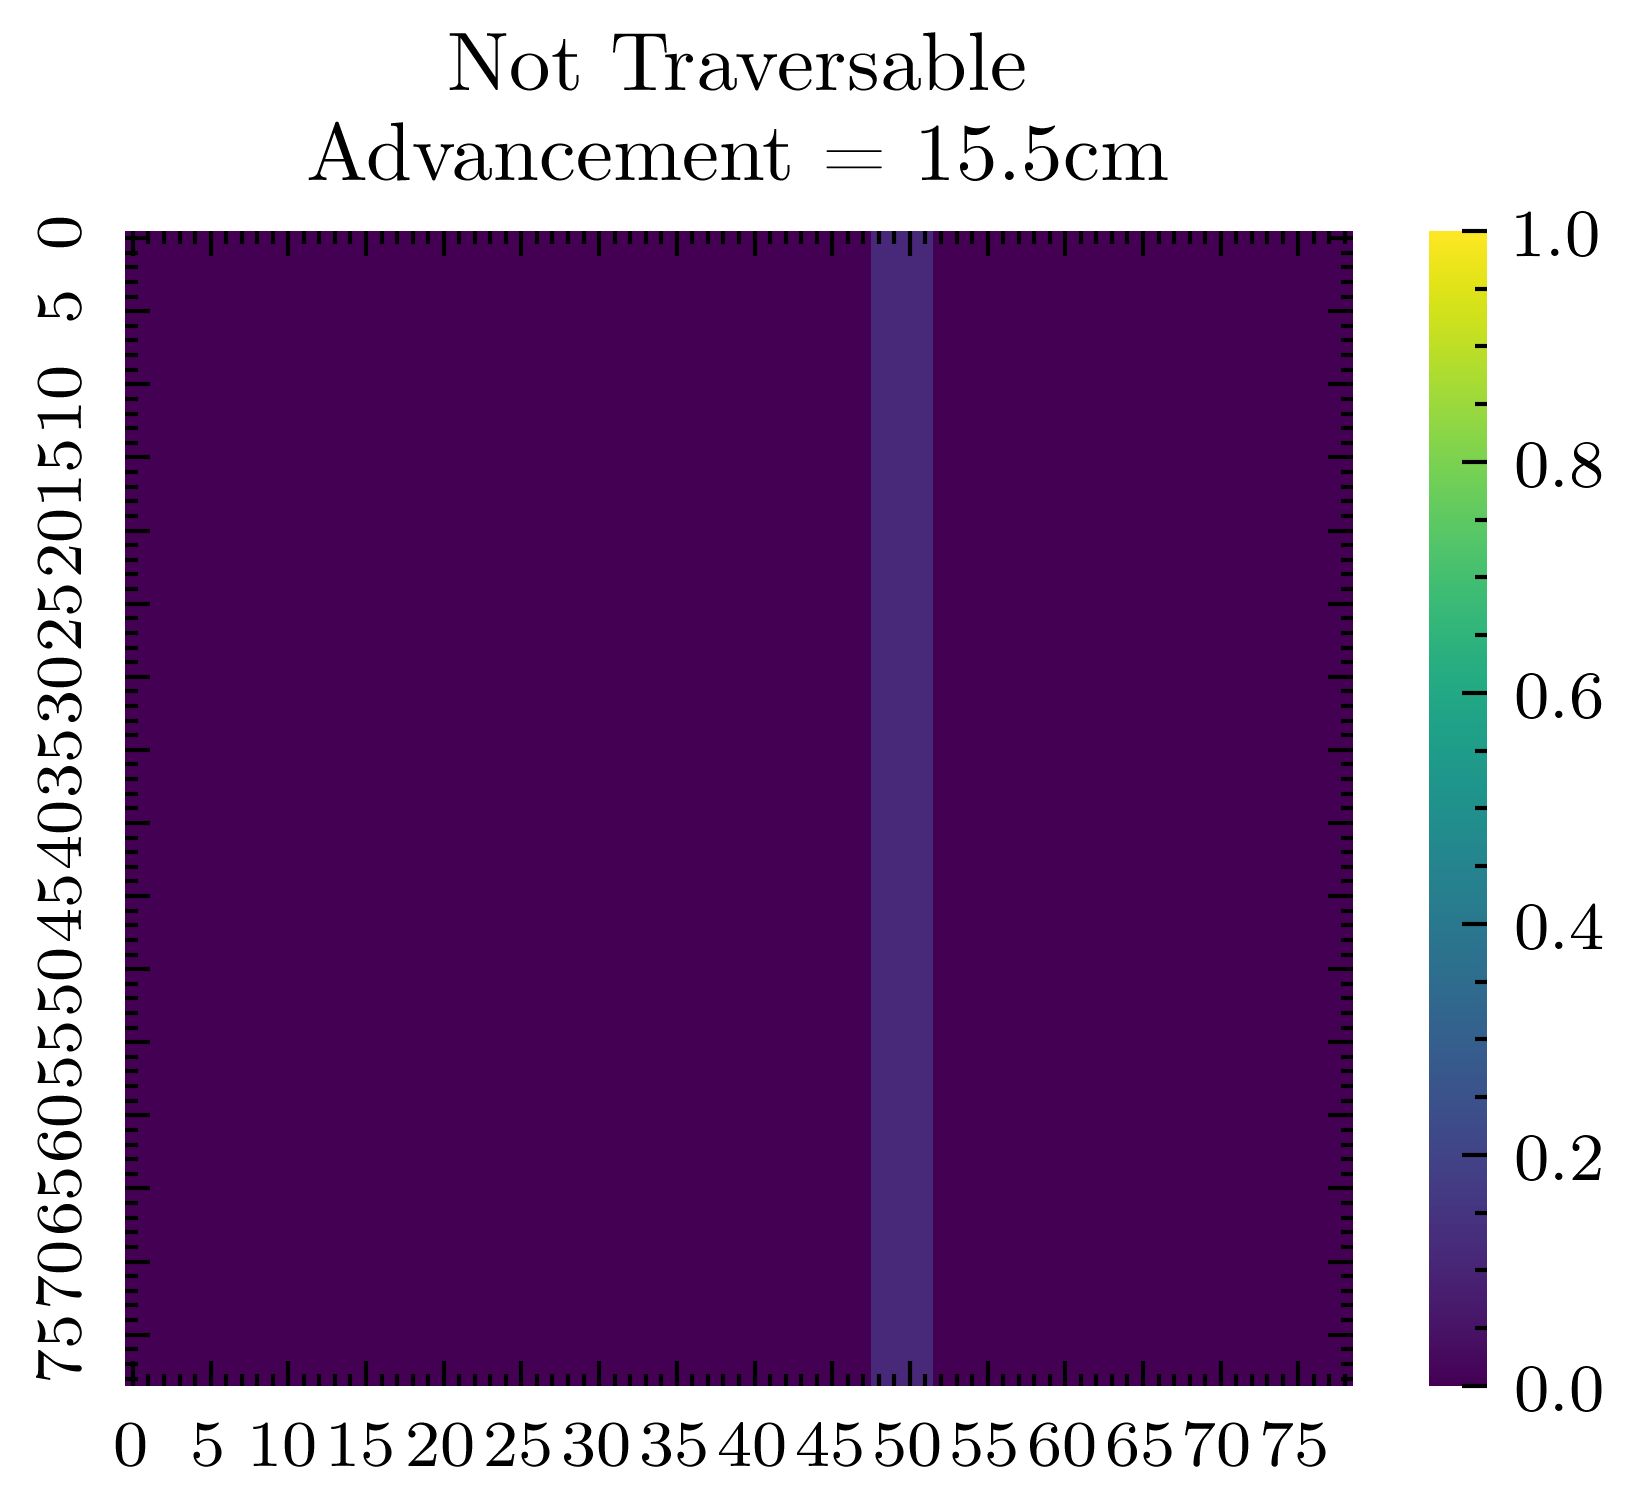
\includegraphics[width=\linewidth]{../img/5/custom_patches/walls_increasing/wall-height-2-2d}
    \end{subfigure}   
    \begin{subfigure}[b]{0.33\textwidth}
        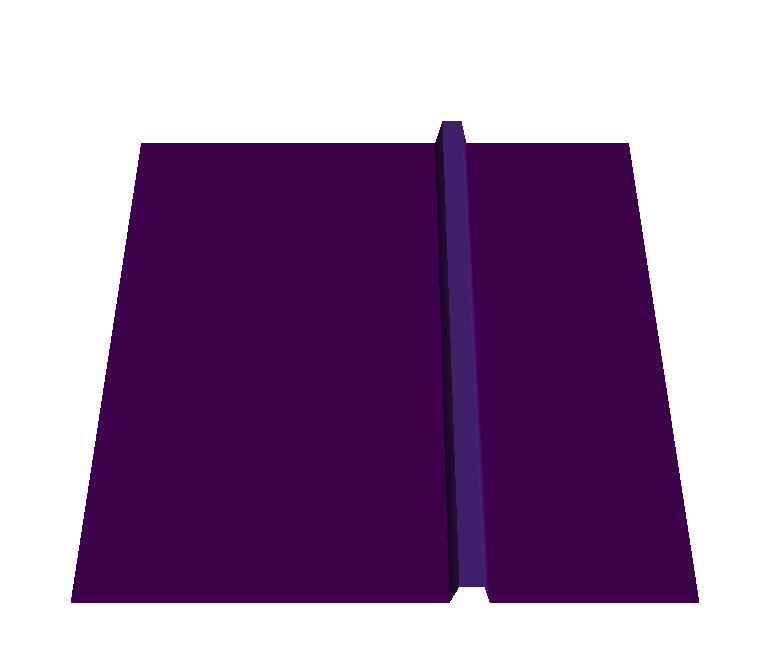
\includegraphics[width=\linewidth]{../img/5/custom_patches/walls_increasing/wall-height-1-3d.png}
    \caption{height $9.7$cm}
    \end{subfigure}   
    \begin{subfigure}[b]{0.33\textwidth}
        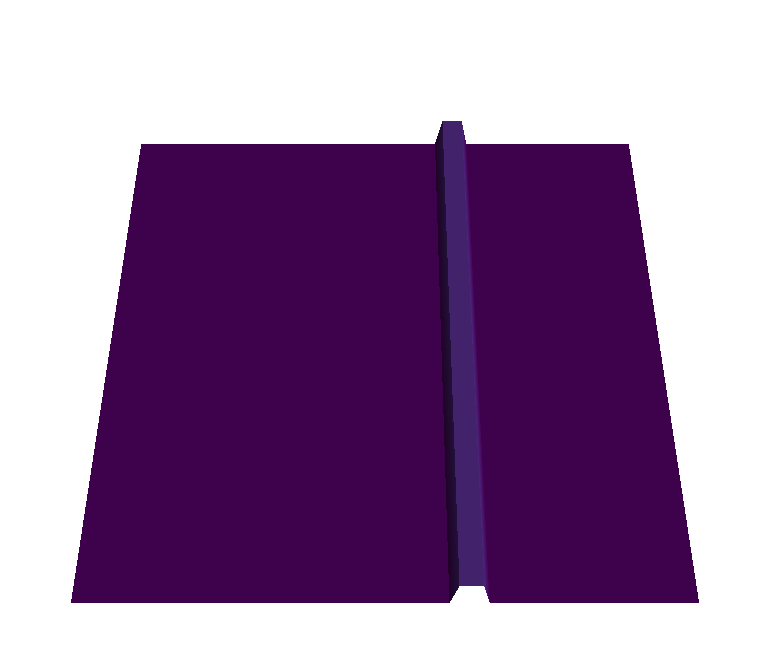
\includegraphics[width=\linewidth]{../img/5/custom_patches/walls_increasing/wall-height-2-3d}
        \caption{height $10$cm}
    \end{subfigure}   
\caption{Patches with a increasing height wall ahead of Krock.}    
\end{figure}
In the first case, the simulator outputs and advancement of $39.5$cm meaning that Krock was able to overcome the obstacle, while in the second case, it was able to traverse just $13.4$cm. Correctly, the predicitons match the real data.

% \subsubsection{Wall under Krock}
% By placing a wall taller than the Krock's distance from the ground the patch won't be traversable anymore since the robot will be lifted up or the back leg wil be stocked. So, as we did in the previous section we created forty patches with a wall from $1$cm to $20$cm in front of the rear legs.

% \begin{figure}[H]
%     \centering
%     \begin{subfigure}[b]{0.160\textwidth}
%     \includegraphics[width=\linewidth]{/home/francesco/Documents/Master-Thesis/papers/Thesis/img/5/custom_patches/wall_under/all/00-3d.png}
%     \end{subfigure}
%     \begin{subfigure}[b]{0.160\textwidth}
%     \includegraphics[width=\linewidth]{/home/francesco/Documents/Master-Thesis/papers/Thesis/img/5/custom_patches/wall_under/all/05-3d.png}
%     \end{subfigure}
%     \begin{subfigure}[b]{0.160\textwidth}
%     \includegraphics[width=\linewidth]{/home/francesco/Documents/Master-Thesis/papers/Thesis/img/5/custom_patches/wall_under/all/10-3d.png}
%     \end{subfigure}
%     \begin{subfigure}[b]{0.160\textwidth}
%     \includegraphics[width=\linewidth]{/home/francesco/Documents/Master-Thesis/papers/Thesis/img/5/custom_patches/wall_under/all/15-3d.png}
%     \end{subfigure}
%     \begin{subfigure}[b]{0.160\textwidth}
%     \includegraphics[width=\linewidth]{/home/francesco/Documents/Master-Thesis/papers/Thesis/img/5/custom_patches/wall_under/all/20-3d.png}
%     \end{subfigure}
%     \begin{subfigure}[b]{0.160\textwidth}
%     \includegraphics[width=\linewidth]{/home/francesco/Documents/Master-Thesis/papers/Thesis/img/5/custom_patches/wall_under/all/25-3d.png}
%     \end{subfigure}
%     \begin{subfigure}[b]{0.160\textwidth}
%     \includegraphics[width=\linewidth]{/home/francesco/Documents/Master-Thesis/papers/Thesis/img/5/custom_patches/wall_under/all/30-3d.png}
%     \end{subfigure}
%     \begin{subfigure}[b]{0.160\textwidth}
%     \includegraphics[width=\linewidth]{/home/francesco/Documents/Master-Thesis/papers/Thesis/img/5/custom_patches/wall_under/all/35-3d.png}
%     \end{subfigure}
%     \caption{Wall under Krock}
%     \end{figure}
    
% The following table summarizes the results
% \begin{table}[H]
%     \centering
%     \begin{tabular}{l|cc}
%         Height(cm) & Prediction \\ 
%         \hline
%         0 - 5cm  & Traversable \\ 
%         5 - end & Not Traversable \\ 
%         \hline
%     \end{tabular}
%     \caption{Model prediction from the wall patches}
% \end{table}
    
\subsection{Tunnel}

\end{document}